\section{Auswertung}
\label{sec:Auswertung}

Die in \autoref{sec:Auswertung} gezeigten Grafiken und Ausgleichsrechnungen sind mithilfe der Python-Bibliotheken Matplotlib \cite{matplotlib}, Scipy \cite{scipy} und Numpy \cite{numpy}
erstellt worden.

\subsection{Überprüfung der Bragg-Bedingung}

Wie in der Durchführung beschrieben wird ein fester Kristallwinkel von $\Theta = 14°$
eingestellt. 
\begin{figure}[H]
  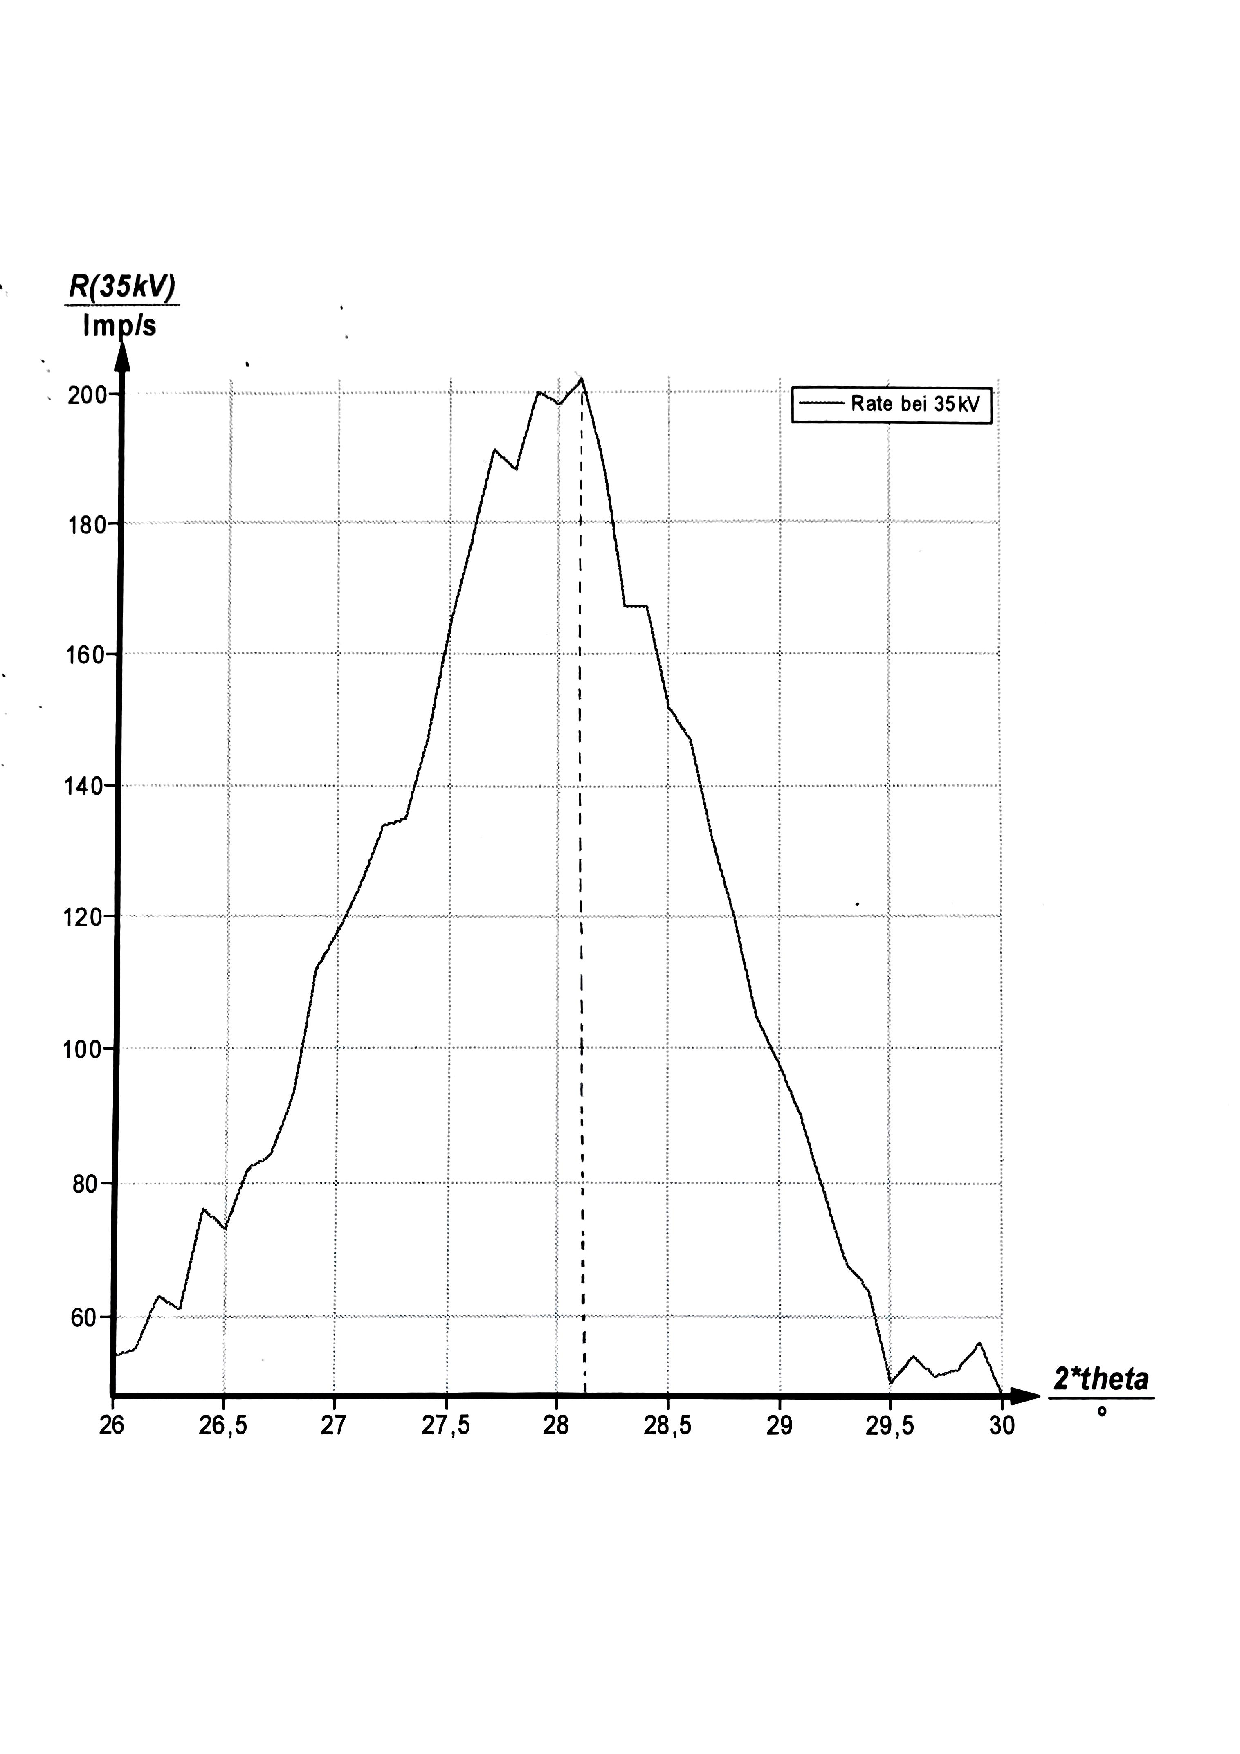
\includegraphics[width=\linewidth]{build/braggbedingung.pdf}
  \caption{...}
  \label{fig:braggbedingung}
\end{figure} 
Das Maximum der Kurve lässt sich aus \autoref{fig:braggbedingung} ablesen:
\begin{equation}
  R_{max} = \SI{203}{Imp/s}.
\end{equation}

\subsection{Das Emissionsspektrum einer Cu-Röntgenröhre}
In \autoref{fig:spektrum} ist der Bremsberg gekennzeichnet. Die K-Linien lassen sich in \autoref{fig:detail} bei 
\begin{align}

\end{align}

\begin{figure}[H]
  \includegraphics[width=\linewidth]{build/bremsberg.pdf}
  \caption{Emissionsspektrum einer Cu-Röntgenröhre.}
  \label{fig:spektrum}
\end{figure}

\begin{figure}[H]
  \includegraphics[width=\linewidth]{build/detail.pdf}
  \caption{Detailspektrum der $K_{\alpha}-$ und $K_{\beta}-$Linie.}
  \label{fig:detail}
\end{figure}
